\section{Deep Belief Networks (DBN)}
Derin İnanç Ağları (Deep Belief Networks), Geoffrey Hinton ve arkadaşları tarafından tanıtılmıştır. Art arda eklenen Kısıtlı Boltzmann Makineleri katmanlarından oluşur. Her alt katmandaki gizli katmanın bir sonraki için görünür katman işlevi görür. Denetimsiz öğrenme yöntemini kullanır. Sadece en üstteki ilk 2 katmanda yönsüz bağlantılar bulunur. 

\begin{figure}[h]
    \centering
    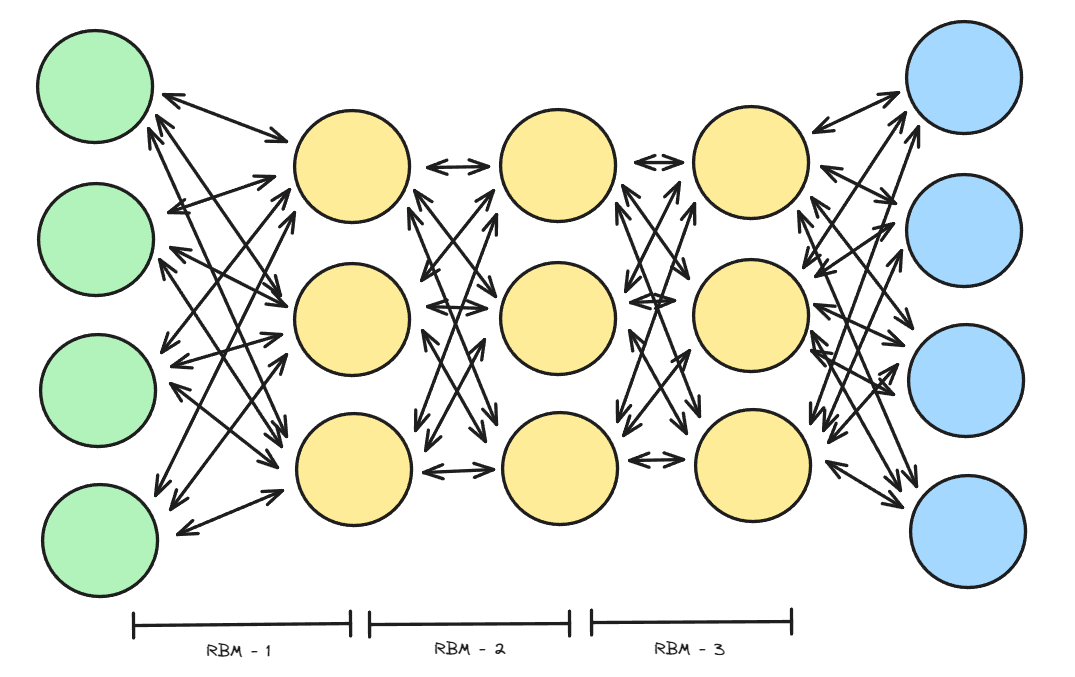
\includegraphics[width=1\textwidth]{images/deep_belief_networks.png}
    \caption{Derin inanç ağı mimarisi.}
    \label{fig:enter-label}
\end{figure}

\newpage